\documentclass{article}
\usepackage[margin=1in]{geometry}

\usepackage{graphicx, booktabs, caption, mathtools, amsfonts, amsthm}
\newtheorem{theorem}{Theorem}[section]
\newtheorem{lemma}[theorem]{Lemma}
\newtheorem{corollary}[theorem]{Corollary}
\newtheorem{example}[theorem]{Example}
\theoremstyle{definition}
\newtheorem{definition}{Definition}[section]
% qed symbo
\renewcommand\qedsymbol{$\blacksquare$}

% no indent
\setlength{\parindent}{0pt}

\usepackage{tikz}
\usetikzlibrary{calc,shapes.geometric}


\title{\LARGE MATH 311 Midterm Summary \\[1em] \normalsize Eddie Guo \\ \today}
\author{}
\date{}

\begin{document}
\maketitle
\vspace{-5em}

\section{Important Equations}

\begin{theorem} \normalfont
    (De Moivre's theorem). $(e^{it})^n = e^{int} \Longrightarrow (\cos t + i \sin t)^n = \cos nt + i \sin nt$.
\end{theorem}

\begin{corollary} \normalfont
    $\cos n \theta = \Re (e^{i n \theta})$ and $\sin n \theta = \Im (e^{i n \theta})$. \vspace{-1.5em}

\begin{align*}
        e^{3i\theta} &= \cos 3 \theta + i \sin 3 \theta = (\cos \theta + i \sin \theta)^3 = \cos^3 \theta + 3i \cos^2 \theta \sin \theta - 3 \cos \theta \sin^2 \theta - i \sin^3 \theta \\
        \Re (e^{3 i \theta}) &= \cos 3 \theta = \cos^3 \theta - 3\cos \theta \sin^2 \theta = \cos^3 \theta - 3 \cos \theta (1-\cos^2 \theta) = 4 \cos^3 \theta - 3\cos \theta \\
        \Im (e^{3 i \theta}) &= \sin 3 \theta = 3\cos^2 \sin \theta - \sin^3 \theta = 3(1 - \sin^3 \theta) \sin \theta - \sin^3 \theta = 3\sin \theta - 4 \sin^3 \theta
    \end{align*}
\end{corollary}

\begin{definition}
    (Complex logs). $\log z = \ln |z| + i \arg z = \ln |z| + i (t + 2 \pi k), k \in \mathbb{Z}$. Furthermore, $z^c = e^{c \log z}$.
\end{definition}

\begin{theorem} \normalfont
    (nth root). If $z^n = c$, then $z = |c|^{1/n} e^{(i \arg c) / n} = |c|^{1/n} e^{i(t + 2\pi k)/n}, \quad k = 0, 1, \dots, n-1$.
\end{theorem}

\begin{example} \normalfont
    Compute $i^{1/3}$. \vspace{-1em}

    \begin{align*}
        i^{1/3} &= e^{\frac{1}{3} \log i} = e^{\frac{1}{3} (\ln |i| + i \arg i)} = e^{\frac{i}{3}} (\pi/2 + 2 \pi k), \quad k = 0, 1, 2 \\
        &\begin{cases}
            k=0: & e^{i\pi/6} = \frac{1}{2} (\sqrt{3} + i) \\
            k=1: & e^{i 5\pi/6} = \frac{1}{2} (-\sqrt{3}+i) \\
            k=2: & e^{i 3\pi/2} = -i
        \end{cases}
    \end{align*}
\end{example}


\section{Trigonometric Functions}

\begin{definition}
    The complex trig functions are
    \begin{align*}
        \cos z &= \frac{e^{iz} + e^{-iz}}{2}, \quad \sin z = \frac{e^{iz} - e^{-iz}}{2i}, \quad \cosh z = \frac{e^z + e^{-z}}{2}, \quad \sinh z = \frac{e^z - e^{-z}}{2} \\
        \cosh z &= \cos iz, \quad i \sinh z = \sin iz, \quad \tanh z = - i \tan iz, \quad \tanh iz = i \tan z \\
        \cos z &= \cos (x+iy) = \cos x \cosh y - i \sin x \sinh y \\
        \sin z &= \sin (x+iy) = \sin x \cosh y + i \cos x \sinh y
    \end{align*}
\end{definition}

\begin{example} \normalfont
    Solve for $z$ given $\cos z = 2$.
    \begin{align*}
        \frac{e^{iz} + e^{-iz}}{2} &= 2 \Longrightarrow e^{2iz} - 4e^{iz} + 1 = 0 \\
        e^{iz} &= \frac{4 \pm \sqrt{16 - 4}}{2} = 2 \pm \sqrt{3} \\
        iz &= \log (2 \pm \sqrt{3}), \quad\quad \text{Note that } (2 + \sqrt{3})(2 - \sqrt{3}) = 1, \text{ so } (2 - \sqrt{3}) = (2 + \sqrt{3})^{-1} \\
        z &= \pm \frac{1}{i} \log (2 + \sqrt{3}) \\
        &= \pm i \log(2 + \sqrt{3}) \\
        &= \pm i \left[ \ln (2 + \sqrt{3}) + i \arg (2 + \sqrt{3}) \right] \\
        &= \pm i \left[ \ln(2 + \sqrt{3}) + i(2\pi k) \right], \quad k \in \mathbb{Z} \\
        &= \pm \left[ i \ln(2 + \sqrt{3}) + 2 \pi k \right], \quad k \in \mathbb{Z}
    \end{align*}
\end{example}


\section{Linear Fractional Transformations (LFTs)}

\begin{definition} \normalfont
    (LFTs). An LFT is defined as $w = w(z) = \frac{az + b}{cz + d}$ where $\det \begin{bmatrix}
        a & b \\ c & d
    \end{bmatrix} \neq 0$.
\end{definition}

\begin{corollary} \normalfont
    Let $w := 1/z$. Then $w$ takes $A(x^2 + y^2) + Bx + Cy + D = 0$ in the $z$-plane to $D(\mu^2 +\nu^2) + B\mu - C\nu + A = 0$ in the $w$-plane, where $w(z) = \mu + i\nu$.
\end{corollary}

\begin{example} \normalfont
    Given $w := 1/z$, what is $|z + 1 - i| = \sqrt{2}$ in the $w$-plane?
    \begin{align*}
        |z + 1 - i| &= \sqrt{2} \Longrightarrow (x+1)^2 + (y-1)^2 = 2 \\
        x^2 + y^2 + 2x - 2y &= 0 \Longrightarrow 2u + 2v + 1 = 0
    \end{align*}
\end{example}

\begin{example} \normalfont
    Given $w := 1/z$, what is $|z-3| = 2$ in the $w$-plane?
    \begin{align*}
        |z-3| &= 2 \Longrightarrow (x-3)^2 + y^2 = 4 \\
        x^2 + y^2 - 6x + 5 &= 0 \Longrightarrow 5(u^2 + v^2) - 6u + 1 = 0 \\
        \left( u - \frac{3}{5} \right)^2 + v^2 &= \left( \frac{2}{5} \right)^2 \Longrightarrow \left| w - \frac{3}{5} \right| = \frac{2}{5}
    \end{align*}
    This is a circle in the $w$-plane centered at $(-3/5, 0)$ with radius $2/5$.
\end{example}

\begin{lemma} \normalfont
    Given $T(P_1) = Q_1,\ T(P_2) = Q_2,\ T(P_3) = Q_3$, we can obtain an LFT $w = w(z)$ by solving
    \begin{equation*}
        \frac{z - P_1}{z - P_3} \left( \frac{P_2 - P_3}{P_2 - P_1 }\right) = \frac{w - Q_1}{w - Q_3} \left( \frac{Q_2 - Q_3}{Q_2 - Q_1 }\right)
    \end{equation*}
\end{lemma}

\begin{lemma} \normalfont
    Given $P_1,\ P_2,\ P_3$ on a circle in $\mathbb{C}$, if $T(P_1)=0,\ T(P_2) = 1,\ T(P_3) = \infty$, then
    \begin{equation*}
        T(z) = \frac{z - P_1}{z - P_3} \left( \frac{P_2 - P_3}{P_2 - P_1} \right)
    \end{equation*}
    maps the circle to the real axis.
\end{lemma}

\begin{theorem} \normalfont
    Compositions of LFTs are LFTs.
\end{theorem}

\begin{example} \normalfont
    Consider the unit circle $\mathcal{C} = |z+i| = 1$. Find an LFT which maps $\mathcal{C}$ to the line $l$ given by the parametric equation $l(t) = (1 + 2i) + t(-2 + i), t \in \mathbb{R}$. Describe the region $w(|z+i| < 1)$. \vspace{1em}

    \begin{minipage}{0.65\textwidth}
        Choose 3 points on $\mathcal{C}:\ 0,\ -2i,\ -1-i$. Set $T(0) = 0$, $T(-2i) = 1$, $T(-1 - i) = \infty$. Then the LFT is
        \begin{equation*}
            T(z) = \frac{z-0}{z - (-1-i)} \left( \frac{-2i - (-1 - i)}{-2i - 0} \right) = \frac{z}{z + 1 + i} \left( \frac{1-i}{-2i} \right) \\
        \end{equation*}
        Since $T(\mathcal{C})$ is the real axis, $l(z) = (-2+i)\ T(z) + (1+2i)$.
    \end{minipage}
    \hfill
    \begin{minipage}{0.3\textwidth}
        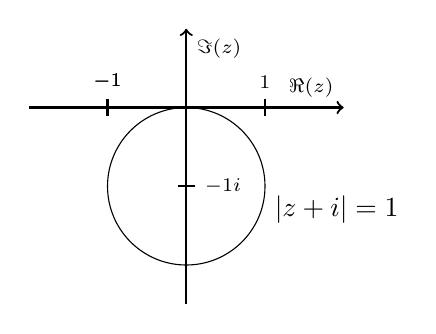
\begin{tikzpicture}
            \begin{scope}[thick,font=\scriptsize]
            % Axes:
            % Are simply drawn using line with the `->` option to make them arrows:
            % The main labels of the axes can be places using `node`s:
            \draw [->] (-2,0) -- (2,0) node [above left]  {$\Re (z)$};
            \draw [->] (0,-2.5) -- (0,1) node [below right] {$\Im (z)$};
        
            % Axes labels:
            % Are drawn using small lines and labeled with `node`s. The placement can be set using options
            \iffalse% Single
            % If you only want a single label per axis side:
            \draw (1,-3pt) -- (1,3pt)   node [above] {$1$};
            \draw (-1,-3pt) -- (-1,3pt) node [above] {$-1$};
            \draw (-3pt,1) -- (3pt,1)   node [right] {$i$};
            \draw (-3pt,-1) -- (3pt,-1) node [right] {$-i$};
            \else% Multiple
            % If you want labels at every unit step:
            \foreach \n in {-1}{%
                \draw (\n,-3pt) -- (\n,3pt)   node [above] {$\n$};
                \draw (-3pt,\n) -- (3pt,\n)   node [right] {$\n i$};
            }
            \fi
            \draw (1, -3pt) -- (1, 3pt) node [above] {$1$};
            \draw (-1, -3pt) -- (-1, 3pt) node [above] {$-1$};
            \end{scope}
            % The circle is drawn with `(x,y) circle (radius)`
            % You can draw the outer border and fill the inner area differently.
            % Here I use gray, semitransparent filling to not cover the axes below the circle
            \path [draw] (0,-1) circle (1);
            % Place the equation into the circle:
            \node [below right] at (+1,-1) {$|z+i| = 1$};
        \end{tikzpicture}
    \end{minipage} \vspace{1em}

    In $(x, y)$ coordinates, $l(t)$ passes through $(1, 2)$ with slope $-1/2: \frac{y-2}{x-1} = -\frac{1}{2} \Longrightarrow y = y(x) = -\frac{1}{2}x + \frac{5}{2}$. Now choose a point within $\mathcal{C}$, say $-i$.
    \begin{align*}
        T(-i) &= \frac{-i}{2i+1} \left( \frac{1-i}{-2i} \right) = \frac{1-i}{4i+2} = -\frac{1}{10} - i \frac{3}{10} \\
        w(-i) &= (-2 + i)\ T(-i) + (1+2i) = (-2 + i) \left( -\frac{1}{10} - i \frac{3}{10} \right) + (1 + 2i) = \frac{3}{2} + i \frac{5}{2} \\
        y(3/2) &= -\frac{1}{2} \left( \frac{3}{2} \right) + \frac{5}{2} = \frac{7}{4} < \frac{5}{2}
    \end{align*}
    Since $w(i)$ is above $l(t)$, $w(|z+i| < 1) = \left\{ z \in \mathbb{C} \mid \Im(z) > - \frac{1}{2} \Re(z) + \frac{5}{2} \right\}$. To find an LFT that maps $l$ to $\mathcal{C}$ (i.e., the inverse map), solve for $z$ in $w = (-2 + i)\ T(z) + (1+2i)$.
\end{example}


\section{Complex Differentiation}

\begin{definition}
    (Complex derivatives). The complex derivative is defined as $f'(z) = \mu_x + i \nu_x = \nu_y - i \mu_y$. The derivative exists $\iff$ the Cauchy-Riemann equations exist: $\mu_x = \nu_y,\ \mu_y = -\nu_x$.
\end{definition}

\begin{definition}
    (Domains). Domains are open, connected sets. Let $D \in \mathbb{C}$ be a domain and $p \in D$ be a point. Then,
    \begin{enumerate}
        \item $f$ is analytic at $p$ if $f'(z)$ exists at $p$ AND in an epsilon neighbourhood around any $p$.
        \item $f$ is analytic $\forall p \in D \iff f'(z)$ is analytic $\forall z \in D$.
        \item $f$ is entire if $f$ is analytic on $\mathbb{C}$.
    \end{enumerate}
\end{definition}

\begin{example} \normalfont
    Let $f(z) = (xy^2 + y) + iyx^2$. Find all points $p \in \mathbb{C}$ where $f'(p)$ exists and compute $f'(p)$. Is $f$ analytic at any $p$? \vspace{1em}

    Let $\mu = xy^2$ and $\nu = yx^2$. By the CR equations,
    \begin{align*}
        \mu_x &= y^2 = x^2 = \nu_y \Longrightarrow x = \pm y \\
        \mu_y &= 2xy + 1 = -2xy = -\nu_x \Longrightarrow xy = -1/4
    \end{align*}
    Therefore, $x = \pm 1/2$ and $y = \mp 1/2$, which means $p = \left\{ \frac{1}{2} (1-i),\ \frac{1}{2} (-1+i) \right\}$.
    \begin{equation*}
        f'(p) = \mu_x(p) + i \nu_x(p) = y^2 + i(2xy) |_p = \frac{1}{4} - \frac{i}{2}
    \end{equation*}
    $f$ is nowhere analytic as $f'$ does not exist on any neighbourhood around $p$.
\end{example}

\begin{example} \normalfont
    Find all points where $f(z) = \frac{\cot z}{z^4 + 16}$ is analytic.
    \begin{align*}
        f(z) &= \frac{\cos z}{\sin z (z^4 + 16)}
        \intertext{Since $\cos z$, $\sin z$, and $z^4 + 16$ are entire, $f$ is analytic except when the denominator is 0.}
        \sin z &= 0 \Longrightarrow z = k \pi, \quad k \in \mathbb{Z} \\
        z^4 + 16 &= 0 \Longrightarrow z = (-16)^{1/4} = 2 e^{i (2m+1) \pi / 4}, \quad m = 0, 1, 2, 3
    \end{align*}
    Thus, $f$ is analytic where $\{ z \in \mathbb{C} \} \setminus \{k\pi,\ 2e^{i \pi/4},\ 2e^{i 3\pi/4},\ 2e^{5\pi/4},\ 2e^{i7\pi/4} \},\ k \in \mathbb{Z}$.
\end{example}

\begin{example} \normalfont
    Let $f(z) = \mu + i \nu$ be an entire function satisfying $A \mu + B \nu + C = 0$, where $z \in \mathbb{C}$, $A, B, C \in \mathbb{R}$, and $(A, B) \neq (0, 0)$. Show that $f \in \mathbb{C}$ is a constant function.
    \begin{align*}
        \begin{rcases}
            A \mu_x + B \nu_x = 0 \\
            A \mu_y + B \nu_y = 0
        \end{rcases} \Longrightarrow
        \begin{bmatrix}
            \mu_x & \nu_x \\ \mu_y & \nu_y
        \end{bmatrix}
        \begin{bmatrix}
            A \\ B
        \end{bmatrix} =
        \begin{bmatrix}
            0 \\ 0
        \end{bmatrix} \Longrightarrow
        \det \begin{bmatrix}
            \mu_x & \nu_x \\ \mu_y & \nu_y
        \end{bmatrix} = \det \begin{bmatrix}
            \mu_x & -\mu_y \\ \mu_y & \mu_x
        \end{bmatrix} = \mu_x^2 + \mu_y^2 = \nu_y^2 + \nu_x^2 = 0
    \end{align*}
    By the CR equations. $\nabla \mu = \nabla \nu = 0$ implies $\mu, \nu \in \mathbb{R}$. Therefore, $f(z) = \mu + i \nu$ is a constant function.
\end{example}

\begin{example} \normalfont
    Let $f(z) = \mu + i \nu$ be an entire function satisfying $\nu = \mu^2$. Show that $f(z) \in \mathbb{C}$ is a constant function.
    \begin{align*}
        \begin{rcases}
            \nu_x = 2 \mu \mu_x \Longrightarrow \nu_x - 2 \mu \mu_x = 0 \\
            \nu_y = 2 \mu \mu_y \Longrightarrow \nu_y - 2 \mu \mu_y = 0
        \end{rcases} \Longrightarrow
        \begin{bmatrix}
            \nu_x & \mu_x \\ \nu_y & \mu_y
        \end{bmatrix}
        \begin{bmatrix}
            1 \\ -2 \mu
        \end{bmatrix} =
        \begin{bmatrix}
            0 \\0
        \end{bmatrix} \\
        \det \begin{bmatrix}
            \mu_x & \nu_x \\ \mu_y & \nu_y
        \end{bmatrix} = \det \begin{bmatrix}
            \mu_x & -\mu_y \\ \mu_y & \mu_x
        \end{bmatrix} = \mu_x^2 + \mu_y^2 = \nu_y^2 + \nu_x^2 = 0
    \end{align*}
    By the CR equations. $\nabla \mu = \nabla \nu = 0$ implies $\mu, \nu \in \mathbb{R}$. Therefore, $f(z) = \mu + i \nu$ is a constant function.
\end{example}


\section{Important Examples}

\begin{example} \normalfont
    $i^{72} - 3i^{81} + 5 = (-1)^{36} - 3(-1)^{40}i + 5 = 6-3i$
\end{example}

\begin{example} \normalfont
    $(1 - \sqrt{3}i)^{-5} = (2e^{-i\pi/3})^{-5} = 2^{-5} e^{i 5 \pi/3} = 2^{-5} \left( \frac{1}{2} - i \frac{\sqrt{3}}{2} \right)$
\end{example}

\begin{example} \normalfont
    $\left| \frac{(3+i)^{20}}{(2-i)^3} \right| = \frac{|3+i|^{20}}{|2-i|^3} = \frac{10^{20/2}}{5^{3/2}} = \frac{10^{10}}{5 \sqrt{5}}$
\end{example}

\begin{example} \normalfont
    Let the roots of the equation $(z+1)^5 + z^5 = 0$ be $z_k,\ k = 0, 1, \dots, 4$. Show that $\Re (z_k) = -1/2$.
    \begin{align*}
        (z+1)^5 + z^5 &= 0 \Longrightarrow \left( -\frac{z+1}{z} \right)^5 = \left( -1 - \frac{1}{z} \right)^5 = 1 \\
        -\left( 1 + \frac{1}{z} \right) &= e^{i (2k\pi/5)}, \quad k = 0, 1, \dots, 4 \Longrightarrow z_k = -\frac{1}{1 + e^{i \lambda k}}, \quad \lambda = 2\pi/5 \\
        &= -\frac{1}{1 + \cos \lambda k + i \sin \lambda k} = -\frac{(1+\cos\lambda k) - i \sin \lambda k}{2(1 + \cos \lambda k)} = -\frac{1}{2} + \frac{i \sin \lambda k}{2 (1 + \cos \lambda k)}
    \end{align*}
    Therefore, $\Re (z_k) = -1/2$ for $k = 0, 1, \dots, 4$, which lies on the line $x = -1/2$.
\end{example}

\begin{example} \normalfont
    Express the complex number $z = \cos (\pi(1+i))$ in the form $a+ib$, where $a, b \in \mathbb{R}$.
    \begin{align*}
        \cos(\pi (1+i)) &= \cos(\pi + i \pi) = \cos \pi \cos i \pi - \sin \pi \sin i \pi \\
        &= \cos \pi \cosh \pi - i \sin \pi \sinh \pi \\
        &= -\cosh \pi \\
        &= -\frac{e^\pi + e^{-\pi}}{2}
    \end{align*}
\end{example}

\begin{example} \normalfont
    $|z|^i = |e^{i \log 2}| = |e^{i (\ln 2 + i \arg 2)}| = |e^{i \ln 2} e^{-2 \pi k}| = e^{-2 \pi k}, \quad k \in \mathbb{Z}$
\end{example}

\begin{example} \normalfont
    Compute $\Re \left[ (1-i \sqrt{3})^{3i} \right]$.
    \begin{align*}
        (1 - i \sqrt{3})^{3i} &= e^{3i \log(1 - i \sqrt{3})} = e^{3i \left[ \ln 2 + i \left( -\frac{\pi}{3} + 2 \pi k \right) \right]} = e^{3i \ln 2} e^{-3 \left( -\frac{\pi}{3} + 2 \pi k \right)}, \quad k \in \mathbb{Z} \\
        &= [\cos (3 \ln 2) + i \sin (3 \ln 2)] e^{\pi - 6 \pi k}, \quad k \in \mathbb{Z} \\
        \Re \left[ (1-i \sqrt{3})^{3i} \right] &= e^{(6k+1) \pi} \cos (3 \ln 2), \quad k \in \mathbb{Z}
    \end{align*}
\end{example}

\begin{example} \normalfont
    Find all values of $\log e^z$.
    \begin{align*}
        \log e^z &= \ln |e^z| + i \arg e^z \\
        |e^z| &= |e^x e^{iy}| = e^x, \quad \arg e^z = \arg (e^x e^{iy}) = y + 2 \pi k, \quad k \in \mathbb{Z} \\
        \log e^z &= \ln e^x + i (y + 2 \pi k) = (x + iy) + 2\pi k i = z + 2 \pi i k, \quad k \in \mathbb{Z}
    \end{align*}
\end{example}

\begin{example} \normalfont
    Show that $\log z^{1/N} = \frac{1}{N} \log z$.
    \begin{align*}
        z^{1/N} &= e^{\log z / N} = e^{\frac{1}{N} (\ln |z| + i \arg z)} = |z|^{1/N} e^{\frac{i}{N} \arg z} \\
        \log z^{1/N} &= \ln |z|^{1/N} + \frac{i}{N} \arg z + 2n \pi i, \quad n \in \mathbb{Z} \\
        &= \frac{1}{N} \ln |z| + \frac{i}{N} \arg z \\
        &= \frac{1}{N} \log z
    \end{align*}
\end{example}

\begin{example} \normalfont
    Show that $\log z^N \neq N \log z$.
    \begin{align*}
        z^N &= e^{N \log z} = e^{N (\ln |z| + i \arg z)} = |z|^N e^{i N \arg z} = |z|^N e^{iN(t + 2 \pi n)}, \quad n \in \mathbb{Z} \\
        \log z^N &= N \ln |z| + i Nt + 2 \pi n i, \quad n \in \mathbb{Z} \\
        &\neq N \ln |z| + i Nt + 2n N \pi i = N \log z
    \end{align*}
\end{example}

\begin{example} \normalfont
    Find all values of $\log[(1+i)^3]$. Are the values the same as that of $3 \log(1+i)$?
    \begin{align*}
        \log[(1+i)^3] &= 3 \ln \sqrt{2} + i \arg [(1+i)^3] = 3 \ln \sqrt{2} + i \left( \frac{3\pi}{4} + 2 \pi n \right), \quad n \in \mathbb{Z} \\
        3 \log(1+i) &= 3 [\ln \sqrt{2} + i \arg (1 + i)] = 3 \ln \sqrt{2} + 3i \left( \frac{\pi}{4} + 2 \pi m \right) = 3 \ln \sqrt{2} + i \left( \frac{3 \pi}{4} + 6 \pi m \right), \quad m \in \mathbb{Z}
    \end{align*}
    Thus, the values are not the same.
\end{example}

\begin{example} \normalfont
    Given $w(z) = \frac{iz+1}{z+i}$.
    \begin{enumerate}
        \item[(i)] Verify that $w(z)$ is an LFT.
 
        $\det \begin{bmatrix}
            i & 1 \\ 1 & i
        \end{bmatrix} = -2 \neq 0$
        \item[(ii)] Describe the image $w(|z| \leq 1)$ in the $w$-plane.
        
        Choose 3 points on the circle $|z| = 1$. Since $w(i) = 0,\ w(-i) = \infty,\ w(1) = 1$, the LFT maps $|z| = 1$ to the real axis, $\Im(z) = 0$. Choose a point inside the circle: $w(0) = -i$. Therefore, $w(|z| \leq 1) = \{ z \in \mathbb{C} \mid \Im(z) \leq 0 \}$.

        \item[(iii)] Find an LFT $w=w(z)$ that takes the real axis to the unit circle $|z|=1$.

        This is the inverse transformation, where we solve for $z$ in terms of $w$:
        \begin{equation*}
            w(z+i) = iz + 1 \Longrightarrow wz - iz = 1 - iw \Longrightarrow z(w-i) = 1 - iw \Longrightarrow z = \frac{1-iw}{w-1} \Longrightarrow w = \frac{-iz + 1}{z-i}
        \end{equation*}
    \end{enumerate}
\end{example}

\begin{example} \normalfont
    Consider the map $w = 1/z$. Describe the image $w(|z+1-2i|) = \sqrt{6}$.
    \begin{align*}
        |z+1-2i| = \sqrt{6} \iff (x+1)^2 + (y-2)^2 &= 6 \iff (x^2+y^2) + 2x - 4y - 1 = 0 \\
        (-1)(\mu^2 + \nu^2) + 2\mu + 4 \nu + 1 &= 0\\
        \mu^2 + \nu^2 - 2\mu - 4\nu - 1 &= 0 \\
        (\mu - 1)^2 + (\nu - 2)^2 &= 6 \\
        |w - 1 - 2i| &= \sqrt{6}
    \end{align*}
    This is a circle in the $w$-plane centered at $(1, 2i)$ with radius $\sqrt{6}$.
\end{example}

\begin{example} \normalfont
    Let $f(z) = 2x^2 - y^2 + i 2xy$.
    \begin{enumerate}
        \item[(i)] Find where the Cauchy-Riemann equations hold.
        \begin{align*}
            \mu_x &= 4x = 2x = \nu_y \Longrightarrow x = 0 \\
            \mu_y &= -2y = \-2y = -\nu_x
        \end{align*}
        Therefore, CR equations hold when $x=0 \Longrightarrow \Re(z) = 0$.
        \item[(ii)] Find where $f$ is differentiable.
 
        The partial derivatives exist and are continuous wherever the CR equations hold. Thus, $f'$ exists and is differentiable when $x = 0$, which implies $\Re(z) = 0$.
        \item[(iii)] Find where the function is analytic.

        $f$ is nowhere analytic because there is no neighbourhood around any point on $\Re(z) = 0$ where $f'$ exists.
    \end{enumerate}
\end{example}

\begin{example} \normalfont
    Find the image of the region $-\frac{\pi}{2} \leq \Im(z) \leq \frac{\pi}{2}$ and $0 \leq \Re(z) \leq 1$ under the transformation $w=e^z$.
    \begin{align*}
        w&= e^z = e^x \cdot e^{iy} = e^x + i e^x \sin y \\
        \mu(x, y) &= e^x \cos y \quad \text{and} \quad \nu(x, y) = e^x \sin y
        \intertext{Holding $x$ fixed at $x=1$, then $\mu^2 + \nu^2 = e^2 (\cos^2 y + \sin^2 y) = e^2$. Thus, the image of the line segment $x=1,\ -\pi/2 \leq y \leq \pi/2$ in the $w$-plane is the semicircle $\mu = e \cos y,\ \nu = e \sin y$, where $y \in [-\pi/2, \pi/2]$.}
        \intertext{Similarly, holding $x$ fixed at $x=0$, then $\mu^2 + \nu^2 = \cos^2 y + \sin^2 y = 1$. Thus, the image of the line segment $x=0,\ -\pi/2 \leq y \leq \pi/2$, in the $w$-plane is the semicircle $\mu = \cos y,\ \nu = \sin y$, where $y \in [-\pi/2, \pi/2]$.}
        \intertext{Holding $y$ fixed at $y=\pi/2$, then $\mu = 0,\ \nu = e^x$, where $0 \leq x \leq 1$. Then the image in the $w$-plane of the line segment $0 \leq x \leq 1,\ y = \pi/2$ is the line segment $\mu=0,\ 1 \leq \nu \leq e$.}
        \intertext{Similarly, holding $y$ fixed at $y=-\pi/2$, then $\mu = 0,\ \nu = -e^x$, where $0 \leq x \leq 1$. Then the image in the $w$-plane of the line segment $0 \leq x \leq 1,\ y = -\pi/2$ is the line segment $\mu=0,\ -e \leq \nu \leq -1$.}
    \end{align*} \vspace{-4em}

    \begin{center}
        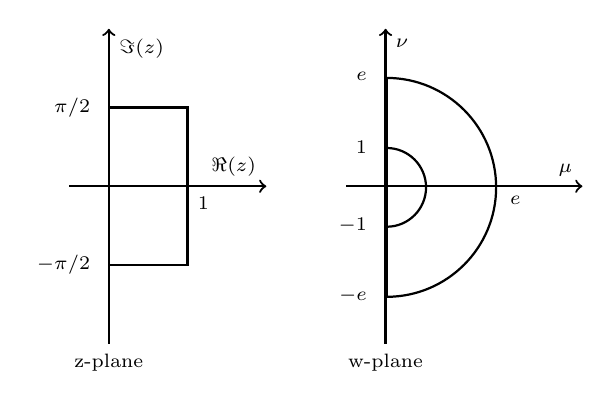
\begin{tikzpicture}
            \begin{scope}[thick,font=\scriptsize]
            % Axes:
            % Are simply drawn using line with the `->` option to make them arrows:
            % The main labels of the axes can be places using `node`s:
            \draw [->] (-0.5,0) -- (2,0) node [above left]  {$\Re (z)$};
            \draw [->] (0,-2) -- (0,2) node [below right] {$\Im (z)$};
    
            % Axes labels:
            \node at (1, 0) [below right] {$1$};
            \node at (-3pt,-1) [left] {$-\pi/2$};
            \node at (-3pt,1) [left] {$\pi/2$};
            \draw[draw=black] (0,-1) rectangle ++(1,2);
            % Place the equation into the circle:
            \node [below] at (0, -2) {z-plane};
            \end{scope}
    
            \begin{scope}[thick,font=\scriptsize,xshift=10em,
                semic/.style args={#1,#2}{semicircle,minimum width=#1,draw,anchor=arc end,rotate=#2}]
            % Axes:
            % Are simply drawn using line with the `->` option to make them arrows:
            % The main labels of the axes can be places using `node`s:
            \draw [->] (-0.5,0) -- (2.5,0) node [above left]  {$\mu$};
            \draw [->] (0,-2) -- (0,2) node [below right] {$\nu$};
    
            % Axes labels:
            \node at (1.65, 0) [below] {$e$};
            \node at (-3pt,-1.39) [left] {$-e$};
            \node at (-3pt,1.39) [left] {$e$};
            \node at (-3pt,-0.5) [left] {$-1$};
            \node at (-3pt,0.5) [left] {$1$};
    
            % semicricle
            \node [semic={2.78cm,270}]at (0,1.39cm){};
            \node [semic={1cm,270}]at (0,0.5cm){};
            % Place the equation into the circle:
            \node [below] at (0, -2) {w-plane};
            \end{scope}
        \end{tikzpicture}
    \end{center}
\end{example}

\end{document}
